\subsubsection{Description}
Cellular neural networks are able to make logical operations on binary pictures, this example shows logical And(Z = -1) and Or(Z = 1)
\subsubsection{Setup}

\textbf{Input 1:} Binary picture\\
\textbf{Initial state/Input 2:} Binary picture.\\
\textbf{Boundary conditions:} Arbitrary (0)\\
\textbf{Output:} Binary.\\
\textbf{Gene:} 1;0;0;0;0;2;0;0;0;0;0;0;0;0;1;0;0;0;0\\


\begin{minipage}{0.9\linewidth}
\begin{equation}
A =
\begin{bmatrix}
 0 &  0 &  0 \\
  0 &  2 &  0 \\
  0 &  0 &  0
\end{bmatrix}
B =
\begin{bmatrix}
 0 & 0 & 0 \\
 0 & 1 & 0 \\
 0 & 0 & 0
\end{bmatrix}
Z = 1
\end{equation}
\captionof{figure}{Chosen values of A,B and Z for this experiment (logical Or)}
\end{minipage}

\subsubsection{Results}
Figure \ref{fig:input1-AO} show input used in this example. The Figure \ref{fig:output-OR} shows typical result of this example, image with negated colors. \\

\begin{minipage}{0.5\linewidth}
	\centering
	
\includegraphics[width=0.9\linewidth]{./Experiments/LogOrAnd/fig/InputV.png} 
	\captionof{figure}{Input1}
	\label{fig:input1-AO}
\end{minipage}
\begin{minipage}{0.5\linewidth}
	\centering
	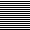
\includegraphics[width=0.9\linewidth]{./Experiments/LogOrAnd/fig/InputH.png}
	\captionof{figure}{Input2}
	\label{fig:input2-AO}
\end{minipage}


\begin{minipage}{0.5\linewidth}
	\centering
	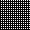
\includegraphics[width=0.9\linewidth]{./Experiments/LogOrAnd/fig/OutputOr.png} 
	\captionof{figure}{Output for OR}
	\label{fig:output-OR}
\end{minipage}
\begin{minipage}{0.5\linewidth}
	\centering
	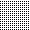
\includegraphics[width=0.9\linewidth]{./Experiments/LogOrAnd/fig/OutputAnd.png}
	\captionof{figure}{output for and}
	\label{fig:output-AN}
\end{minipage}
